\subsection{dijet mass turn-on}
\label{section: dijet mass turn-on}

The lowest single jet un-prescaled trigger in 2015 was HLT\_j360, in 2016 was HLT\_j380,
in 2017 and 2018 is HLT\_j420 which is avaliable in full Run 2 data.
The trigger selection will will bias the mass spectrum at low mass region, to avoid this bias, so an additional mass cut will be appied. 

To measure the $m_{jj}$ turn-on in data, an unbiased sample was obtained using the HLT\_j360 trigger, only data collected in 2015 corresponding to 3.2 $fb^{-1}$ is used in this measuerment.

Figure \ref{fig: mass turn-on yStar 0.6} shows the efficiencies as a function of $m_{jj}$ for $|y^{*}|<0.6$ in two g-tag regions, applying directly either triggers, respectively. The $m_{jj}$ value of the plateau ($\geq$99.5\%) is 1100 GeV. Figure \ref{fig: mass turn-on yStar 0.8} shows the efficiencies as a function of $m_{jj}$ for $|y^{*}|<0.8$ in two g-tag regions, the plateau value is 1200 GeV.

\begin{figure}[htbp]
        \centering
        \subfigure[$\geq$1 g-tag]{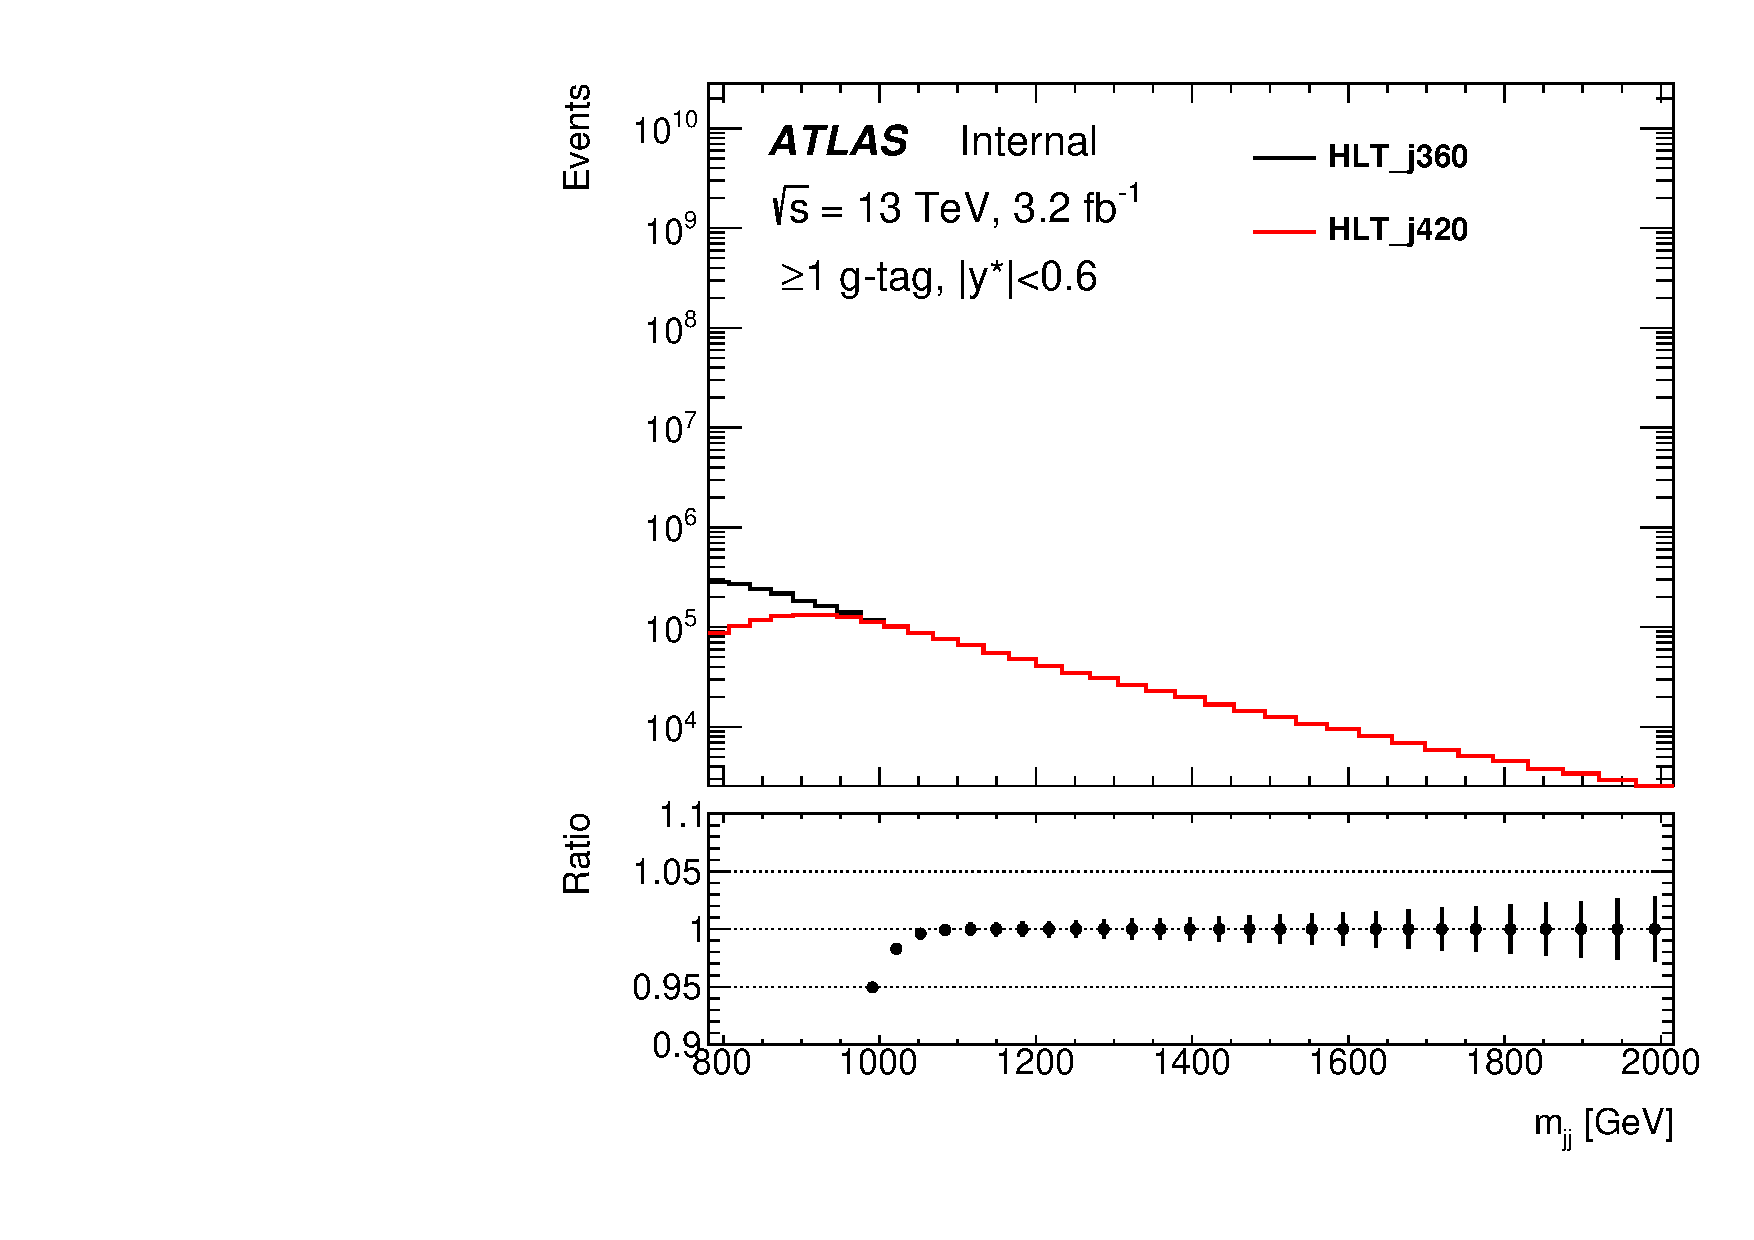
\includegraphics[width=0.48\columnwidth]{figures/massturnon/h_mass_gj_yStar0p6_ratio.pdf}}
        \subfigure[2 g-tag]{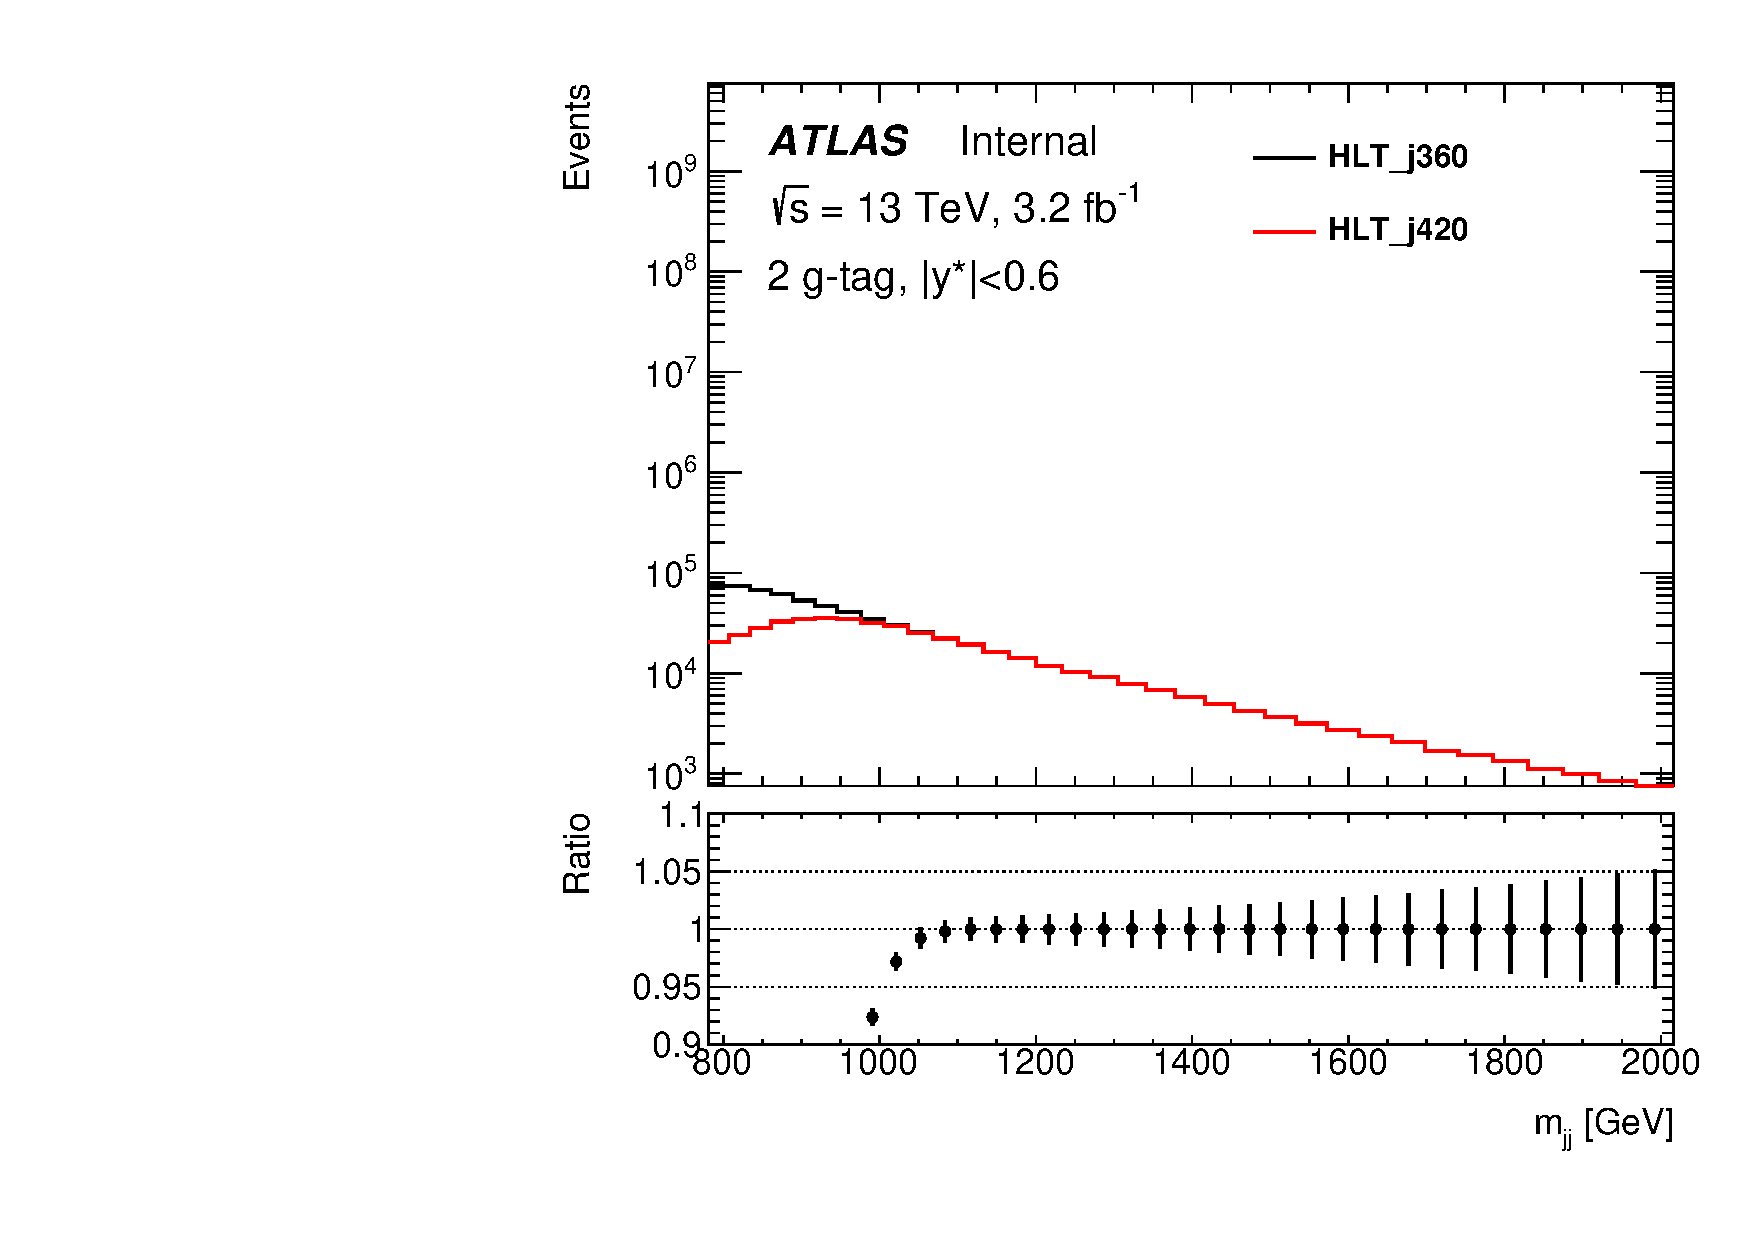
\includegraphics[width=0.48\columnwidth]{figures/massturnon/h_mass_gg_yStar0p6_ratio.pdf}}
        \caption{Efficiencies as a function of $m_{jj}$ for $y^{*}|<0.6$ using HLT\_j420 in the case of (a) $\geq$1 g-tag, (b) 2 g-tag.}
        \label{fig: mass turn-on yStar 0.6}
\end{figure}

\begin{figure}[htbp]
        \centering
        \subfigure[$\geq$1 g-tag]{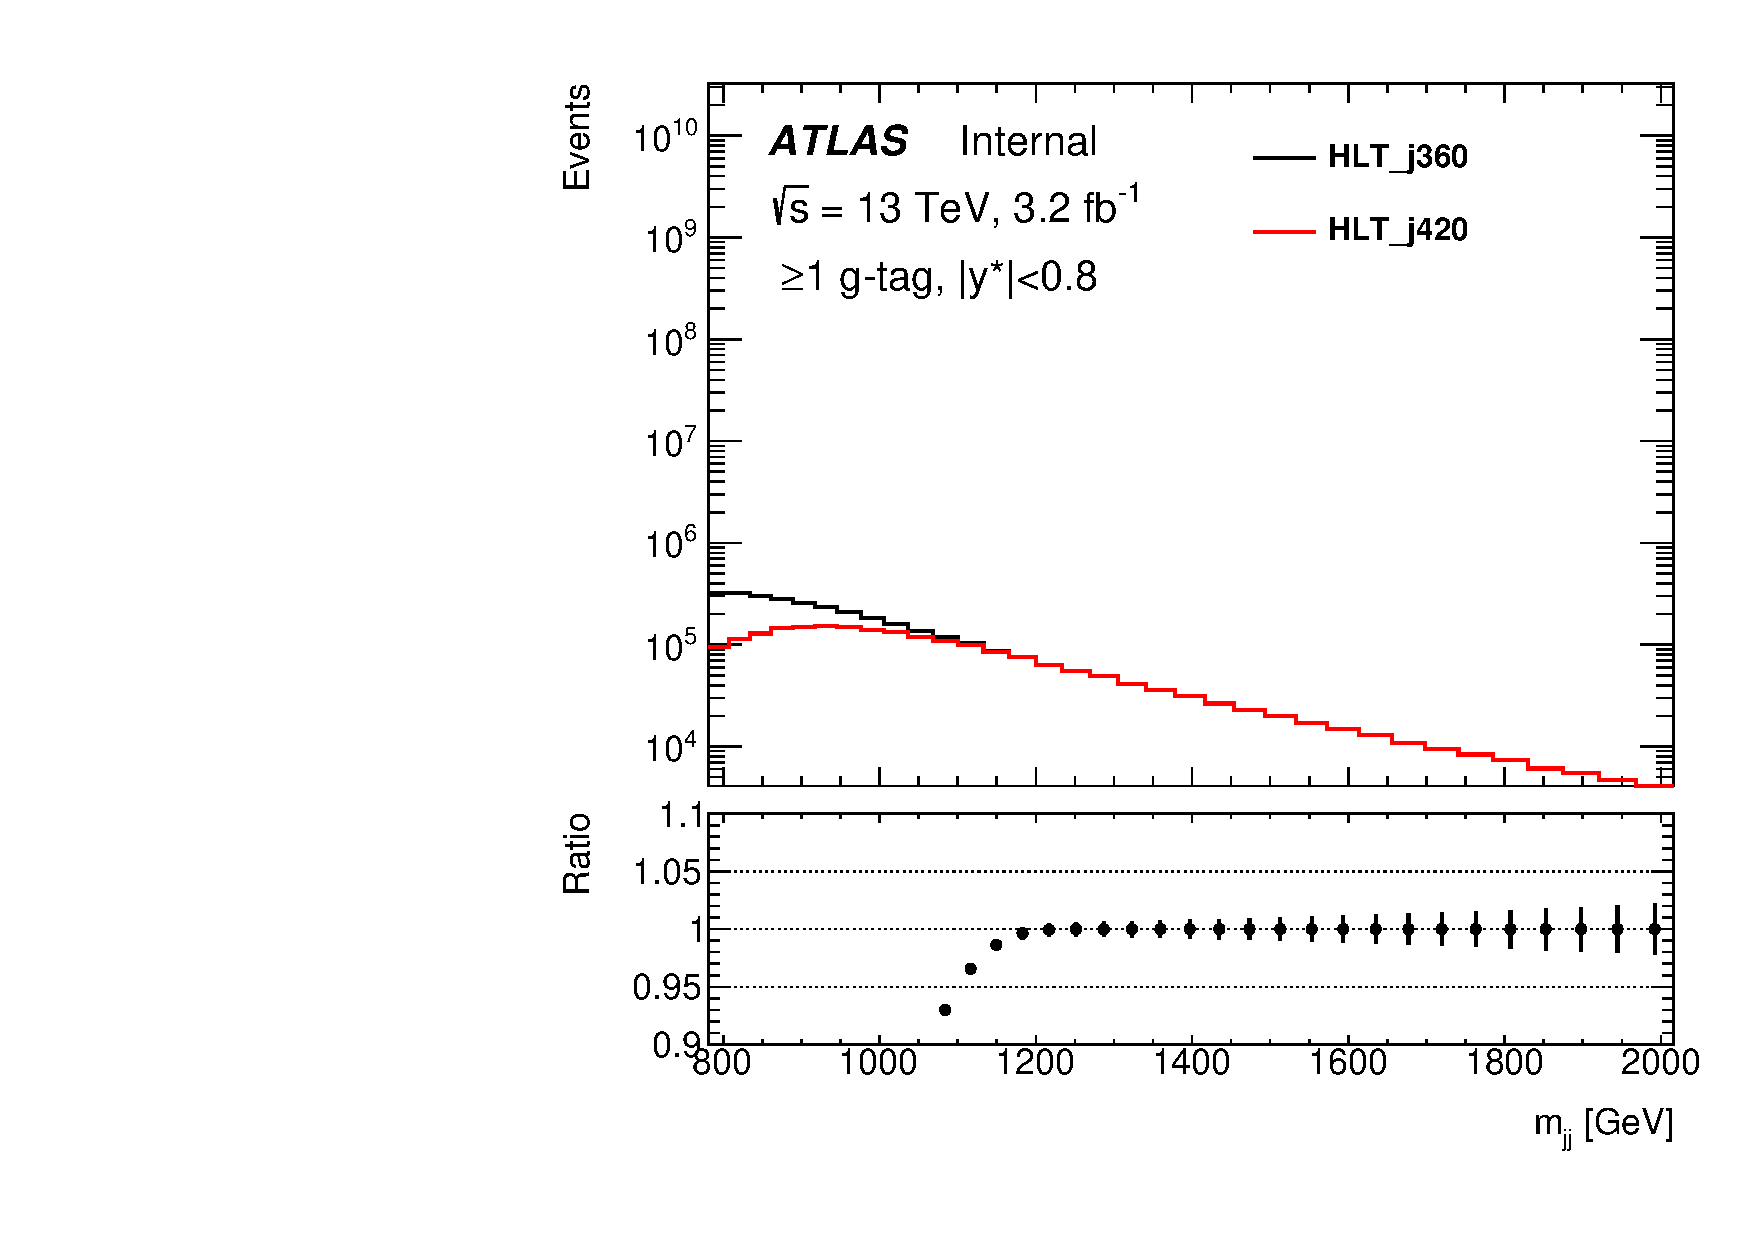
\includegraphics[width=0.48\columnwidth]{figures/massturnon/h_mass_gj_yStar0p8_ratio.pdf}}
        \subfigure[2 g-tag]{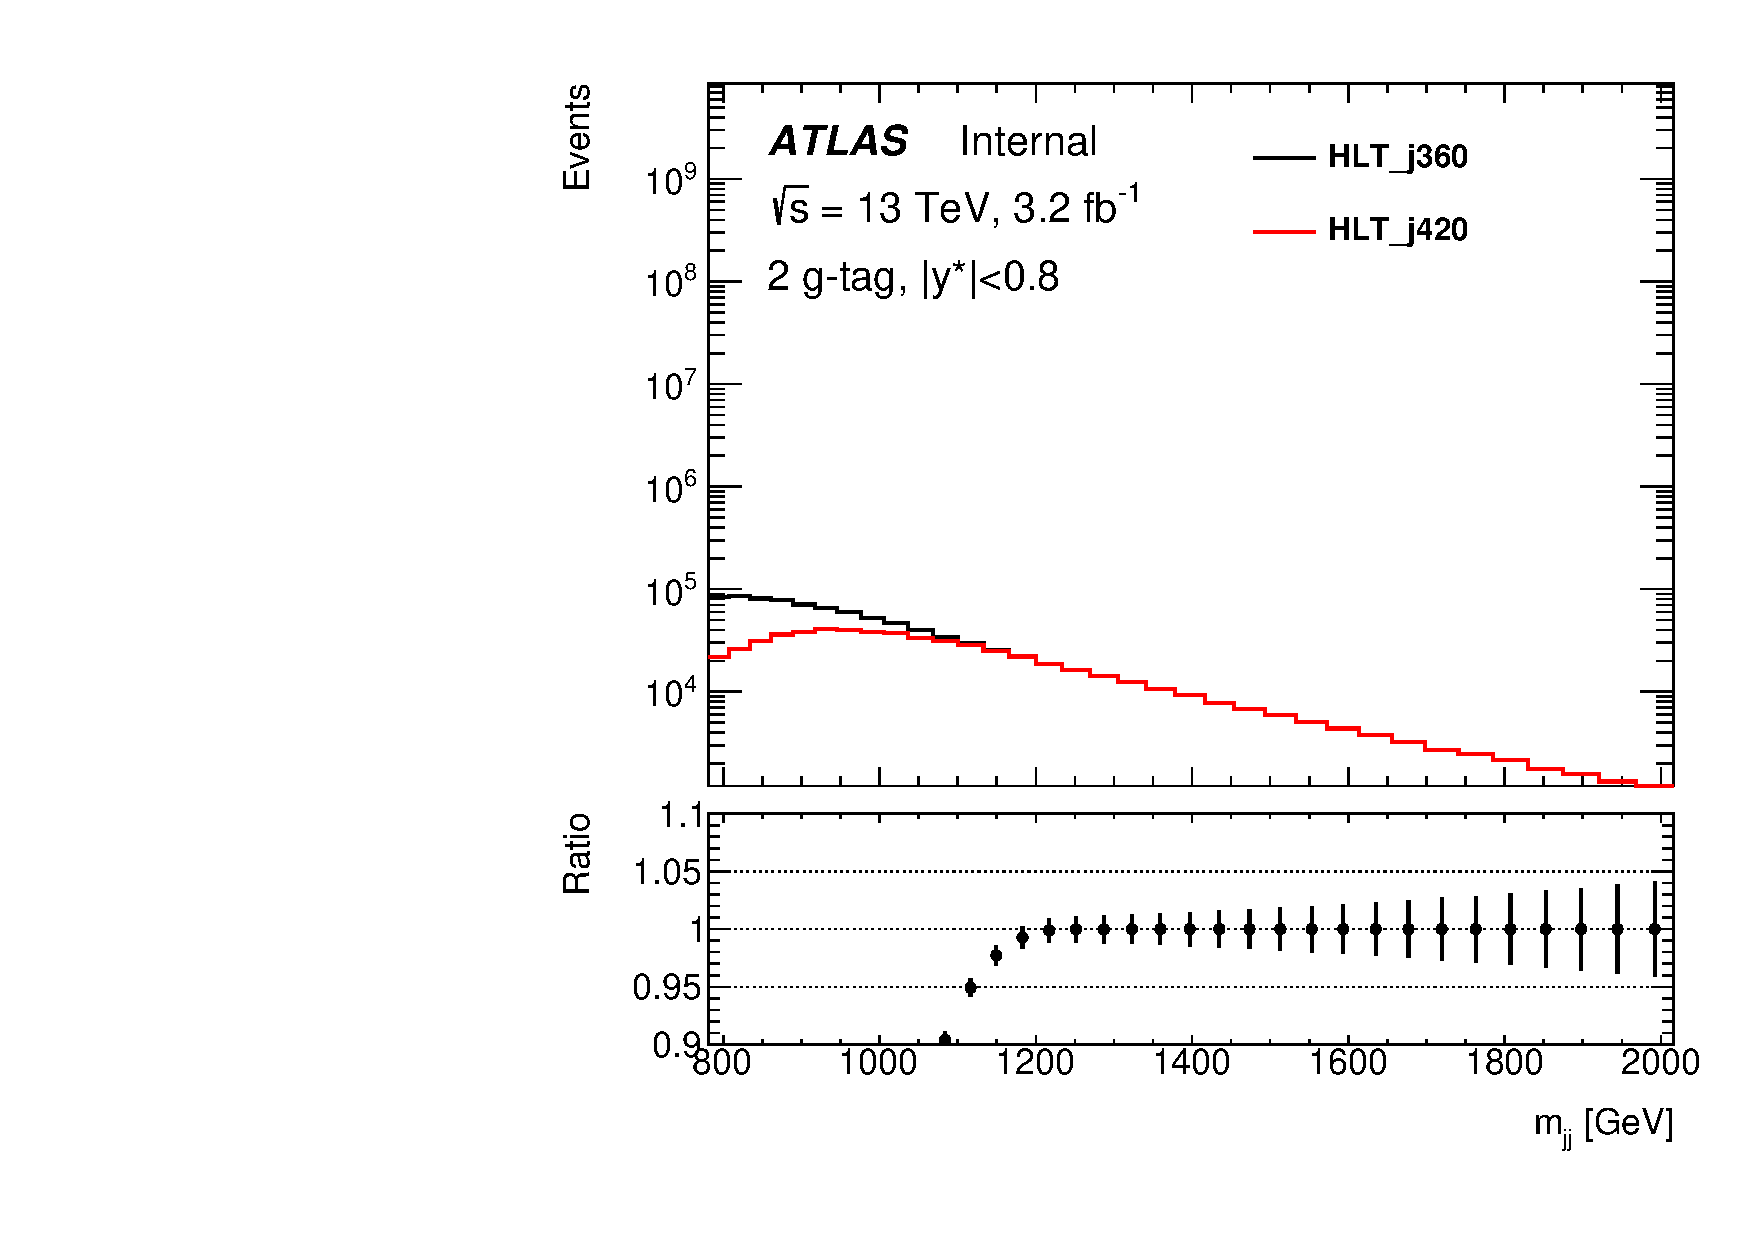
\includegraphics[width=0.48\columnwidth]{figures/massturnon/h_mass_gg_yStar0p8_ratio.pdf}}
        \caption{Efficiencies as a function of $m_{jj}$ for $y^{*}|<0.8$ using HLT\_j420 in the case of (a) $\geq$1 g-tag, (b) 2 g-tag.}
        \label{fig: mass turn-on yStar 0.8}
\end{figure}
